\documentclass[a4paper, 10pt, ]{article}

\usepackage[slovak]{babel}

% ------------------------------

\usepackage[utf8]{inputenc}
\usepackage[T1]{fontenc}

\usepackage[left=4cm,
            right=4cm,
            top=2.1cm,
            bottom=2.6cm,
            footskip=7.5mm,
            twoside,
            marginparwidth=3.0cm,
            %showframe,
            ]{geometry}

\usepackage{graphicx}
\usepackage[dvipsnames]{xcolor}
% https://en.wikibooks.org/wiki/LaTeX/Colors

% ------------------------------

\usepackage{lmodern}

\usepackage[tt={oldstyle=false,proportional=true,monowidth}]{cfr-lm}
% https://mirror.szerverem.hu/ctan/fonts/cfr-lm/doc/cfr-lm.pdf

% ------------------------------

\usepackage{amsmath}
\usepackage{amssymb}
\usepackage{amsthm}

\usepackage{booktabs}
\usepackage{multirow}
\usepackage{array}
\usepackage{dcolumn}

\usepackage{natbib}

% ------------------------------

\hyphenpenalty=6000
\tolerance=1000

\def\naT{\mathsf{T}}

% ------------------------------

\makeatletter

    \def\@seccntformat#1{\protect\makebox[0pt][r]{\csname the#1\endcsname\hspace{4mm}}}

    \def\cleardoublepage{\clearpage\if@twoside \ifodd\c@page\else
    \hbox{}
    \vspace*{\fill}
    \begin{center}
    \phantom{}
    \end{center}
    \vspace{\fill}
    \thispagestyle{empty}
    \newpage
    \if@twocolumn\hbox{}\newpage\fi\fi\fi}

    \newcommand\figcaption{\def\@captype{figure}\caption}
    \newcommand\tabcaption{\def\@captype{table}\caption}

\makeatother

% ------------------------------

\usepackage{fancyhdr}
\fancypagestyle{plain}{%
\fancyhf{} % clear all header and footer fields
% \fancyfoot[C]{\sffamily {\bfseries \thepage}\ | {\scriptsize\oznacenieCasti}}
\fancyfoot[C]{\sffamily {\bfseries \thepage}{\color{Gray}\scriptsize$\,$z$\,$\pageref{LastPage}}\ | 
\includegraphics[height=5pt]{../../COMMONFILES/KUT_logo_v0.1.pdf}{\scriptsize\KUTporadoveCislo}}
\renewcommand{\headrulewidth}{0pt}
\renewcommand{\footrulewidth}{0pt}}
\pagestyle{plain}

% ------------------------------

\usepackage{titlesec}
\titleformat{\paragraph}[hang]{\sffamily  \bfseries}{}{0pt}{}
\titlespacing*{\paragraph}{0mm}{3mm}{1mm}
\titlespacing*{\subparagraph}{0mm}{3mm}{1mm}

\titleformat*{\section}{\sffamily\Large\bfseries}
\titleformat*{\subsection}{\sffamily\large\bfseries}
\titleformat*{\subsubsection}{\sffamily\normalsize\bfseries}


% ------------------------------

\PassOptionsToPackage{hyphens}{url}
\usepackage[pdfauthor={},
            pdftitle={},
            pdfsubject={},
            pdfkeywords={},
            % hidelinks,
            colorlinks=false,
            breaklinks,
            ]{hyperref}


% ------------------------------

\graphicspath{%
{../fig_standalone/}%
{../../PY/fig/}%
{../../ML/fig/}%
{./fig/}%
}

% ------------------------------

\usepackage{enumitem}

\usepackage{lettrine}

% ------------------------------

\usepackage{lastpage}

\usepackage{microtype}

% ------------------------------

\usepackage{algorithm}
\usepackage[noend]{algpseudocode}
\makeatletter
\renewcommand{\ALG@name}{Algoritmus}
\makeatother
\usepackage{amsmath}
\usepackage{bbold}
\usepackage{calc}
\usepackage{dsfont}
\usepackage{mathtools}
\usepackage{tabto}


\newcommand{\mr}[1]{\mathrm{#1}}
\newcommand{\bs}[1]{\boldsymbol{#1}}
\newcommand{\bm}[1]{\mathbf{#1}}

\newcommand{\diff}[2]{\frac{\Delta #1}{\Delta #2}}
\newcommand{\der}[2]{\frac{d #1}{d #2}}
\newcommand{\parder}[2]{\frac{\partial #1}{\partial #2}}

\newcommand{\argmax}[0]{\mr{argmax}}
\newcommand{\diag}[0]{\mr{diag}}
\newcommand{\rank}[0]{\mr{rank}}
\newcommand{\trace}[0]{\mr{tr}}

\renewcommand{\Re}{\mr{Re}}
\renewcommand{\Im}{\mr{Im}}


\theoremstyle{definition}
\newtheorem{definition}{Definícia}[section]
\newtheorem{theorem}{Veta}[section]
\newtheorem{lemma}[theorem]{Lemma}
\newtheorem{example}{Príklad}[section]
\renewcommand*{\proofname}{Dôkaz}

% ------------------------------


% -----------------------------------------------------------------------------

\def\oznacenieCelku{Kolekcia učebných textov}

% -----------------------------------------------------------------------------


\def\KUTporadoveCislo{dev250820}

\def\oznacenieVerzie{v0.9}
% \def\oznacenieVerzie{\phantom{v1.0}}

\def\mesiacRok{august 2025}

\def\authorslabel{MT}






% -----------------------------------------------------------------------------

\begin{document}

% -----------------------------------------------------------------------------
% Uvodny nadpis

\noindent
\parbox[t][18mm][c]{0.3\textwidth}{%
\raisebox{-0.9\height}{%
\phantom{.}
\includegraphics[height=18mm]{./COMMONFILES/URKFEIlogo.pdf}%
}%
}%
\parbox[t][18mm][c]{0.7\textwidth}{%
\raggedleft

\sffamily
\fontsize{16pt}{18pt}
\fontseries{sbc}
\selectfont

\noindent
\textcolor[rgb]{0.75, 0.75, 0.75}{\textls[25]{\oznacenieCelku}}
}%

\noindent
\parbox[t][16mm][b]{0.5\textwidth}{%
\raggedright

\color{Gray}
\sffamily

\fontsize{12pt}{12pt}
\selectfont
\mesiacRok

\fontsize{6pt}{10pt}
\selectfont
\href{https://github.com/OkoliePracovnehoBodu/KUT}{github.com/OkoliePracovnehoBodu/KUT}

\fontsize{8pt}{10pt}
\selectfont
\authorslabel




}%
\parbox[t][16mm][b]{0.5\textwidth}{%
\raggedleft

\sffamily

\fontsize{6pt}{6pt}
\selectfont

\textcolor[rgb]{0.68, 0.68, 0.68}{\oznacenieVerzie}


\fontsize{14pt}{14pt}
\selectfont

\bfseries


\includegraphics[height=12pt]{./COMMONFILES/KUT_logo_v0.1.pdf}%
{%
\textls[-50]{\KUTporadoveCislo}
}%
}%

% -----------------------------------------------------------------------------




\vspace{6mm}

% ---------------------------------------------
\sffamily
\bfseries
\fontsize{18pt}{21pt}
\selectfont

\begin{flushleft}
    Laboratórne zariadenie TS:\\ orientačný prehľad
\end{flushleft}

\bigskip

% -----------------------------------------------------------------------------
\normalsize
\normalfont
% -----------------------------------------------------------------------------

\lstset{style=mystyle}










\noindent
\lettrine[lines=1, nindent=1pt, loversize=0.0]{C}{ieľom} 
textu je opis laboratórneho zariadenia TS predstavujúceho fyzický model spojitého dynamického systému.


\section{Opis dynamického systému}

TS, skratka od \emph{tepelný systém} (thermal system), je laboratórne zariadenie predstavujúce reálny dynamický systém. Pozostáva zo sklenenej trubice umiestnenej na podstave. Na jednom konci trubice je upevnený ventilátor, ktorý do trubice vháňa vzduch. V trubici hneď za ventilátorom sa nachádza výhrevné teleso (výhrevná špirála). Za špirálou je umiestnený prvý teplotný snímač a druhý je umiestnený na opačnom konci trubice. V~podstave sa nachádza elektronika zabezpečujúca napájanie komponentov zariadenia a~rozhranie k meracej karte.

Dostupnými sú dva vstupné a dva výstupné analógové signály. Prvý vstupný signál ovláda výkon vyhrievacieho telesa. Druhý vstupný signál ovláda výkon ventilátora. Prvý výstupný signál je teplota vzduchu v~trubici hneď za vyhrievacím telesom. Druhý výstupný signál je teplota vzduchu v trubici na opačnom konci od vyhrievacieho telesa.

Z kybernetického hľadiska je zariadenie TS možné prevádzkovať ako mnohovstupový a~mnohovýstupový systém (MIMO systém) alebo ako jednovstupový a jedno výstupový systém (SISO systém). 

Pri SISO systéme je vstupom signál ovládajúci výkon vyhrievacieho telesa. Signál pre ventilátor v podstate určuje prevádzkovú podmienku alebo prevádzkové nastavenie zariadenia keďže prúdenie vzduchu v trubici vo všeobecnosti vplýva na jeho ohrievanie a teplotu.





\section{Rozsahy a jednotky signálov}

Z opisu predmetného dynamického systému plynie, že systém ma dva vstupné a dva výstupné signály.

Všetky štyri signály nadobúdajú hodnoty v~rozsahu $0$ až $10$ pričom ide o~napäťové signály vo voltoch [V].

Signál ovládajúci výkon vyhrievacieho telesa označme vstup~1~a~signál ovládajúci výkon ventilátora označme vstup~2. Signál zo snímača teploty hneď za vyhrievacím telesom označme výstup~1 a~signál zo snímača teploty na opačnom konci trubice označme výstup~2.

\begin{center}

\vspace{-10pt}    
    
\tabcaption{Rozsahy a jednotky signálov}
\label{tab:rozsahy_a_jednotky_signalu}

\lstyle

\begin{tabular*}{\textwidth}{@{ \extracolsep{\fill}} lll}
\toprule
Signál & Rozsah hodnôt & Jednotka \\
\midrule
Vstup 1 & $0$ až $10$ & V (volt) \\
Vstup 2 & $0$ až $10$ & V (volt) \\
Výstup 1 & $0$ až $10$ & V (volt) \\
Výstup 2 & $0$ až $10$ & V (volt) \\
\bottomrule
\end{tabular*}


\end{center}













\section{Schematické znázornenie systému}


\begin{center}

    \vbox{%


        \makebox[\textwidth][c]{%
        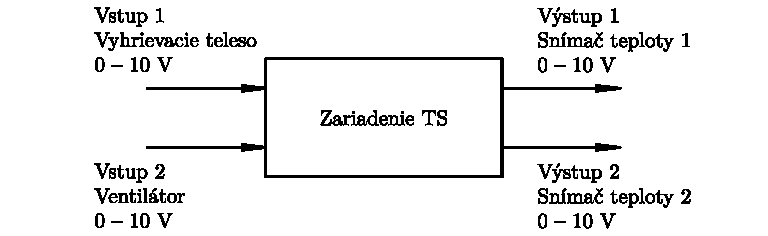
\includegraphics{TS_sch1.pdf}
        }

        \figcaption{ 
            Signály systému TS.
        }
        \label{TS_sch1}
    }%vbox

\end{center}


\begin{center}

    \vbox{%


        \makebox[\textwidth][c]{%
        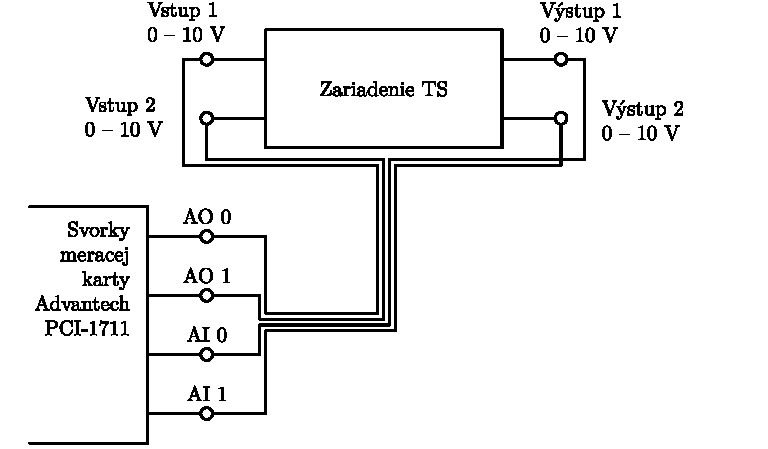
\includegraphics{TS_sch2b.pdf}
        }

        \figcaption{ 
            Schéma pripojenia laboratórneho zariadenia k svorkám meracej karty Advantech PCI-1711, pričom AO~$0$ a AO~$1$ sú analógové výstupy meracej karty a~AI~$0$, AI~$1$ sú analógové vstupy meracej karty.
        }
        \label{TS_sch2b}
    }%vbox

\end{center}



\section{Fotografie}

Zoznam fotografií:

\begin{itemize}[leftmargin=0pt, labelsep=3mm, itemsep=0pt]
    \item Obr. \ref{IMG_5575_toPDF}: Celkový pohľad na laboratórne zariadenie TS.
    \item Obr. \ref{IMG_5589_toPDF}: Detail na sklenenú trubicu laboratórneho zariadenia TS.
    \item Obr. \ref{TS_sch3_foto}: Pohľad zhora s vyznačením jednotlivých komponentov.   
\end{itemize}

\noindent
\vbox{%

    \makebox[\textwidth][c]{%
    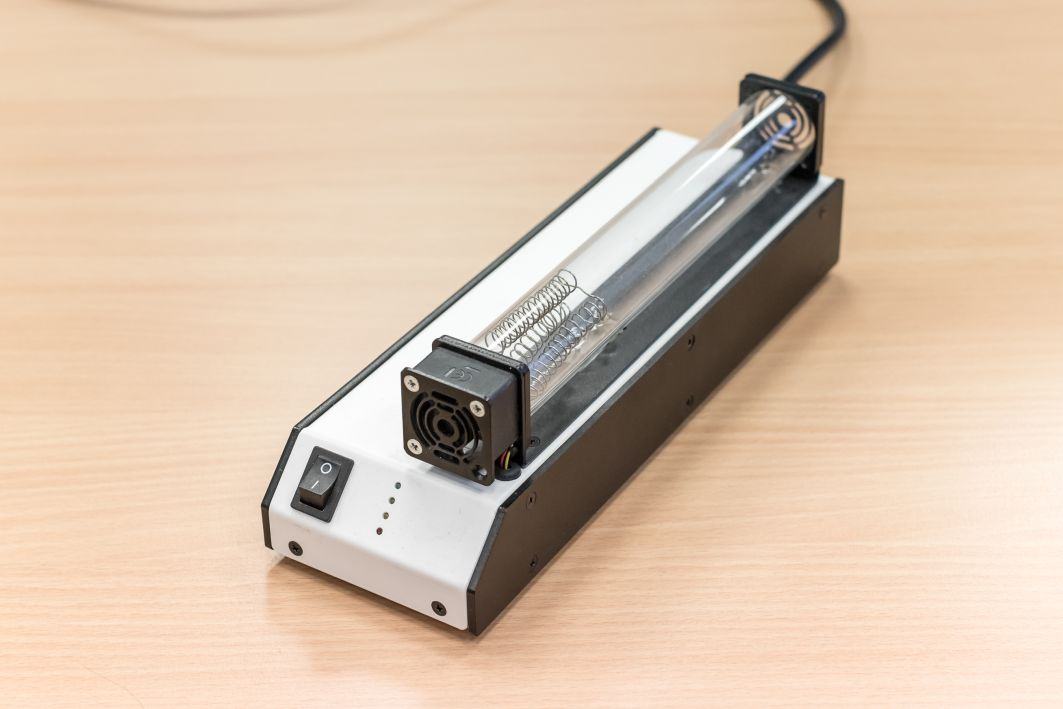
\includegraphics{IMG_5575_toPDF.jpg}
    }

    \figcaption{ 
        Celkový pohľad na laboratórne zariadenie TS.
    }
    \label{IMG_5575_toPDF}
}%vbox

\vfill

\noindent
\vbox{%

    \makebox[\textwidth][c]{%
    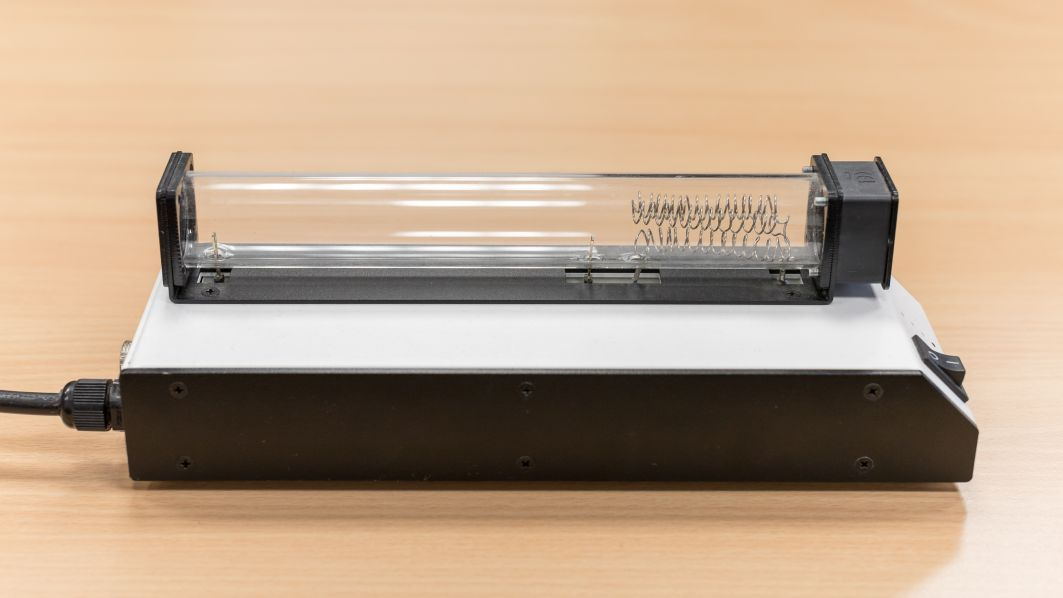
\includegraphics{IMG_5589_toPDF.jpg}
    }

    \figcaption{ 
        Detail na sklenenú trubicu laboratórneho zariadenia TS. 
    }
    \label{IMG_5589_toPDF}
}%vbox


\bigskip

\noindent
\vbox{%

    \makebox[\textwidth][c]{%
    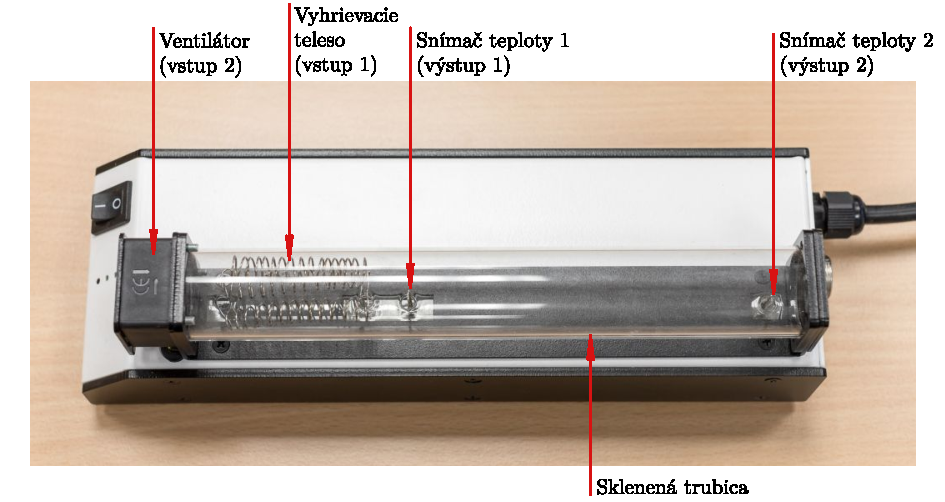
\includegraphics{TS_sch3_foto.pdf}
    }

    \figcaption{ 
        Pohľad zhora s vyznačením jednotlivých komponentov. 
    }
    \label{TS_sch3_foto}
}%vbox

































































% -----------------------------------------------------------------------------

\end{document}

% -----------------------------------------------------------------------------